\section{Experiments}
In this section we experimentally verify the RRP algorithm with various input parameters. For this we used a Intel Core i7 2.66 GHz processor with 8GB RAM and running MAC OSX. 

We use real Yelp Dataset\footnote{https://www.yelp.com/dataset\_challenge} which has both social and spatial components as introduced in the beginning. The dataset has 552K social nodes, 77K spatial nodes, 3.5M social edges and 2.2M spatial edges. As social edges indicate friendship strength between users, we generate a random number between 1 to 10 to signify the social distance between two users. Similarly, as every spatial edge is a check-in at a business, we indicate the rating given by the user by a random number between 1 and 10. In both cases larger the number, lower is the friendship strength and lower is the rating respectively. 

Unless specified each run uses the default parameter values shown in table \ref{tab:default-param}. Parameter K is the shorthand for top-k, i.e. any query requests 160 shortest paths by default. RZ is the shorthand for resolution which determines the number of blocks the world is divided into. RZ $\gets$ 100 implies that the world is equally into 100 by 100 blocks along latitudes and longitudes. \textit{VertexReachesAlgo} parameter defines how the function LIES\_IN is implemented. We had three implementations which check whether the query region R overlaps with regions reachable from a vertex. We will describe each type near those experiments. M and RF are the same parameters described before as the size of the index and reduction factor between each level of the index.

In all the algorithms, the DisjointSearch approach first filters nodes based on spatial constraint and finds the shortest path to each using a well known shortest path algorithm called Dijkstra's until K paths are found.

\begin{table}[h]
	\caption{Default parameter values}
	\label{tab:default-param}
	\begin{center}
		\renewcommand{\arraystretch}{1.25}
		\begin{tabular}{ l | l | l }
			\hline
			Parameter & Value & Range \\ \hline
			\hline
			K & 160 & 10, 20, 40, 80, 160, 320, 640, 1280 \\
			RZ & 100 & 10, 100, 500, 1000, 5000 \\
			VertexReachesAlgo & Type 3 & Type 1, Type 2, Type 3 \\
			M & 10K & Any positive integer \\
			RF & 4 & Any positive integer \\
			\hline
		\end{tabular}
	\end{center}
\end{table}

\begin{figure}[t]
	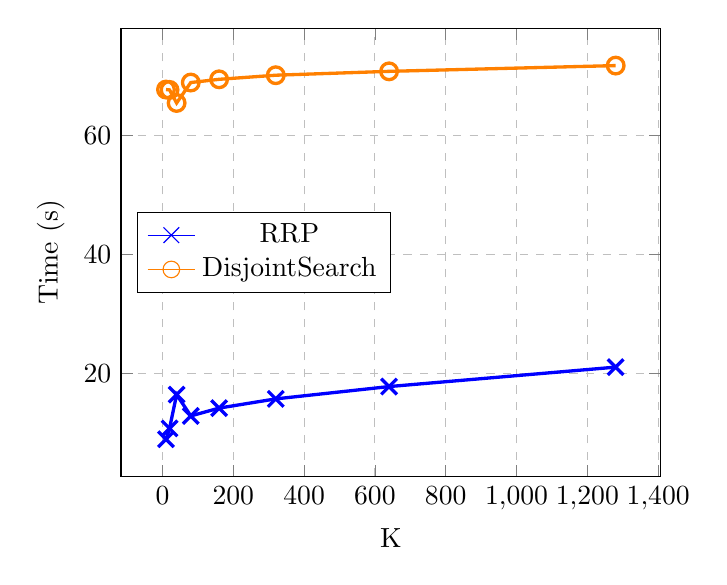
\begin{tikzpicture}[every plot/.append style={very thick}]
	\begin{axis}[
	    xlabel={K},
	    ylabel={Time (s)},
	    legend style={at={(0.03,0.5)},anchor=west},
	    xmajorgrids=true,
	    ymajorgrids=true,
	    % xtick={0, 10, 20, 40, 80, 160, 320, 640, 1280},
	    % xticklabel style={rotate=90},
	    grid style=dashed,
	    % axis line style = ultra thin
	]
	 
	\addplot[
	    color=blue,
	    mark=x,
	    mark size=4pt
	    ]
	    coordinates {
	    (10,8.91)(20,10.72)(40,16.41)(80,12.82)(160,14.14)(320,15.69)(640,17.76)(1280,21.03)
	    };
	\addplot[
	    color=orange,
	    mark=o,
	    mark size=3pt
	    ]
	    coordinates {
	    (10,67.72)(20,67.66)(40,65.46)(80,68.9)(160,69.44)(320,70.13)(640,70.78)(1280,71.75)
	    };
	    \legend{RRP, DisjointSearch}
	 
	\end{axis}
	\end{tikzpicture}
	\caption{Runtime comparison between DisjointSearch and RRP algorithms}
	\label{fig:plot-01}
\end{figure}

Figure \ref{fig:plot-01} compares the time taken by RRP and DisjointSearch approach for the same source vertex and region. The DisjointSearch approach totally takes a disconnected approach between spatial and social constraints while RRP does a joint search in both the domains using a heuristic. As K increases, the time taken also increases linearly. Though it may be very unlikely that we query for K $>$ 20, RRP still outperforms DisjointSearch approach by at least 3 times even in the worst cases. To be specific, the region in the query has 2,804 spatial nodes and we set K as high as 1,280 nodes (viz. 50\%) in that region which is very unlikely and testing the limits. Now that we know the final outcome, lets split the RRP into components and analyze each. As RRP is made of Spatial Index and Social Index, we can run RRP multiple times with and without each index.

\begin{figure*}[t]
	\begin{subfigure}[t]{0.33\textwidth}
		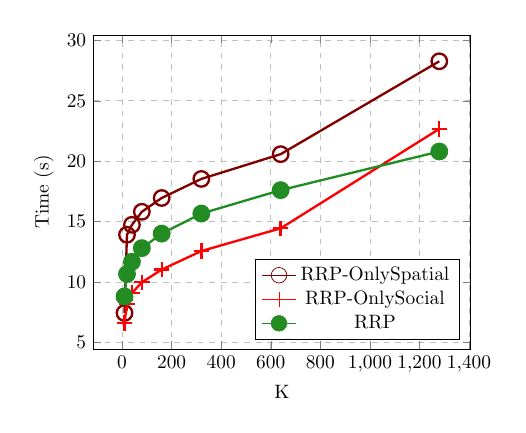
\begin{tikzpicture}[every plot/.append style={very thick}, scale=0.70]
			\begin{axis}[
			    xlabel={K},
			    ylabel={Time (s)},
			    legend pos=south east,
			    xmajorgrids=true,
			    ymajorgrids=true,
			    grid style=dashed,
			   	mark size=4pt
			]
			 
			%\addplot[
			%    color=blue,
			%    mark=x,
			%    ]
			%    coordinates {
			%    (10,73.8)(20,64.22)(40,64.06)(80,64.66)(160,69.06)(320,69.48)(640,64.44)(1280,64.44)
			%    };
			\addplot[
			    color=Maroon,
			    mark=o,
			    ]
			    coordinates {
			    (10,7.43)(20,13.91)(40,14.73)(80,15.81)(160,16.95)(320,18.53)(640,20.58)(1280,28.27)
			    };
			\addplot[
			    color=red,
			    mark=+,
			    ]
			    coordinates {
			    (10,6.62)(20,8.2)(40,9.08)(80,9.97)(160,11.02)(320,12.56)(640,14.44)(1280,22.67)
			    };
			\addplot[
			    color=ForestGreen,
			    mark=*,
			    ]
			    coordinates {
			    (10,8.8)(20,10.66)(40,11.67)(80,12.8)(160,14)(320,15.66)(640,17.6)(1280,20.8)
			    };
			%    \legend{DisjointSearch, RRP-OnlySpatial, RRP-OnlySocial, RRP}
			    \legend{RRP-OnlySpatial, RRP-OnlySocial, RRP}
			 
			\end{axis}
		\end{tikzpicture}
		% \caption{Runtime comparison between DisjointSearch and types of RRP algorithms for RZ = 10}
		\caption{Runtime comparison between the types of RRP algorithms for RZ = 10}
		\label{fig:plot-02}
	\end{subfigure}
	\begin{subfigure}[t]{0.33\textwidth}
		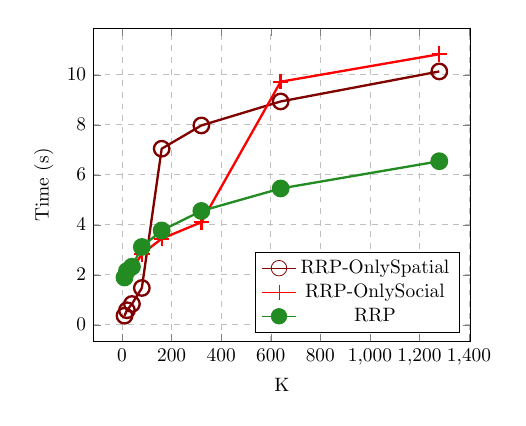
\begin{tikzpicture}[every plot/.append style={very thick}, scale=0.70]
			\begin{axis}[
			    xlabel={K},
			    ylabel={Time (s)},
			    legend pos=south east,
			    xmajorgrids=true,
			    ymajorgrids=true,
			    grid style=dashed,
			    mark size=4pt
			]
			 
			% \addplot[
			%     color=blue,
			%     mark=x,
			%     ]
			%     coordinates {
			%     (10.0, 33.54)(20.0, 25.28)(40.0, 30.72)(80.0, 30.07)(160.0, 29.89)(320.0, 24.95)(640.0, 24.93)(1280.0, 30.34)
			%     };
			\addplot[
			    color=Maroon,
			    mark=o,
			    ]
			    coordinates {
			    (10.0, 0.36)(20.0, 0.58)(40.0, 0.83)(80.0, 1.47)(160.0, 7.04)(320.0, 7.97)(640.0, 8.93)(1280.0, 10.13)
			    };
			\addplot[
			    color=red,
			    mark=+,
			    ]
			    coordinates {
			    (10.0, 1.85)(20.0, 2.19)(40.0, 2.19)(80.0, 2.83)(160.0, 3.44)(320.0, 4.1)(640.0, 9.72)(1280.0, 10.82)
			    };
			\addplot[
			    color=ForestGreen,
			    mark=*,
			    ]
			    coordinates {
			    (10.0, 1.89)(20.0, 2.15)(40.0, 2.32)(80.0, 3.11)(160.0, 3.77)(320.0, 4.55)(640.0, 5.45)(1280.0, 6.54)
			    };
			    % \legend{DisjointSearch, RRP-OnlySpatial, RRP-OnlySocial, RRP}
			    \legend{RRP-OnlySpatial, RRP-OnlySocial, RRP}
			 
			\end{axis}
		\end{tikzpicture}
		% \caption{Runtime comparison between DisjointSearch and types of RRP algorithms for RZ = 100}
		\caption{Runtime comparison between the types of RRP algorithms for RZ = 100}
		\label{fig:plot-09}
	\end{subfigure}
	\begin{subfigure}[t]{0.33\textwidth}
		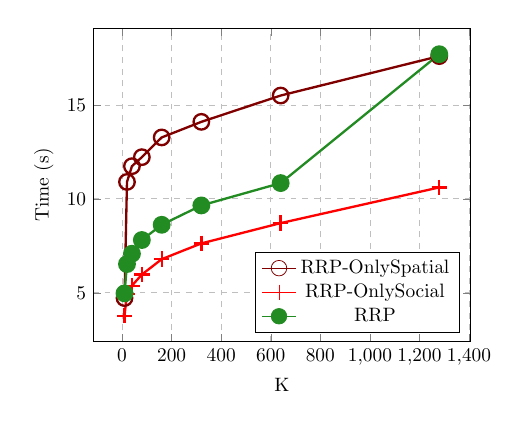
\begin{tikzpicture}[every plot/.append style={very thick}, scale=0.70]
			\begin{axis}[
			    xlabel={K},
			    ylabel={Time (s)},
			    legend pos=south east,
			    xmajorgrids=true,
			    ymajorgrids=true,
			    grid style=dashed,
			    mark size=4pt
			]
			 
			% \addplot[
			%     color=blue,
			%     mark=x,
			%     ]
			%     coordinates {
			%     (10,32.23)(20,29.95)(40,24.9)(80,30.6)(160,24.82)(320,29.76)(640,24.97)(1280,25)
			%     };
			\addplot[
			    color=Maroon,
			    mark=o,
			    ]
			    coordinates {
			    (10,4.72)(20,10.9)(40,11.74)(80,12.22)(160,13.27)(320,14.1)(640,15.5)(1280,17.6)
			    };
			\addplot[
			    color=red,
			    mark=+,
			    ]
			    coordinates {
				(10,3.78)(20,4.94)(40,5.38)(80,5.97)(160,6.79)(320,7.63)(640,8.71)(1280,10.61)
			    };
			\addplot[
			    color=ForestGreen,
			    mark=*,
			    ]
			    coordinates {
			    (10,4.97)(20,6.53)(40,7.08)(80,7.81)(160,8.62)(320,9.65)(640,10.84)(1280,17.7)
			    };
			    % \legend{DisjointSearch, RRP-OnlySpatial, RRP-OnlySocial, RRP}
			    \legend{RRP-OnlySpatial, RRP-OnlySocial, RRP}
			 
			\end{axis}
		\end{tikzpicture}
		% \caption{Runtime comparison between DisjointSearch and types of RRP algorithms for RZ = 1,000}
		\caption{Runtime comparison between the types of RRP algorithms for RZ = 1,000}
		\label{fig:plot-03}
	\end{subfigure}
	\caption{Runtime comparison between the types of RRP algorithms for different resolutions}
\end{figure*}


So Figure \ref{fig:plot-02} breaks down the components of RRP into RRP-OnlySpatial, RRP-OnlySocial and Both with resolution of 10 by 10. RRP-OnlySpatial implies we use only the Spatial index and perform a search. Though using either of the indices beat DisjointSearch algorithm, we can now clearly see in this case using RRP-OnlySocial index outperforms others. To understand why this is the case, we have to revisit how our heuristic algorithm works. Our heuristic function uses the Social index with landmark(s). Combined with triangle inequality we get a lower bound on the distance between the current vertex along the path and a destination vertex in the region. If the lower bound is tight, we get increase the pruning power of RRP. As discussed the quality of landmark(s) plays an important role in the performance. So here using the spatial index we are only adding the overhead by querying that index, therefore the curve using both the indices is slightly underperforming. This can happen again if graph is really dense as in our case that the spatial index will mostly answer yes for reachability queries. Therefore bottom line, using social index only gives better results when:
\begin{itemize}
  \item Quality of the heuristic, indirectly landmarks, is very good
  \item Graph is very dense that most of the vertices can reach the region
\end{itemize}

However, we can see that as the value of K increases, using both the indices certainly helps as un-necessary graph traversals are further reduced by spatial index and its over head is overcome. We will see this clearer in a later Figure when the quality of the landmark is not as good as this case. We used a very low resolution of 10 by 10 and so lets see how the runtimes change when we increase it by 100 times.

% \begin{figure}

% \end{figure}

Just as expected as shown in Figure \ref{fig:plot-03}, the gap between Both and RRP-OnlySocial indices further increases when resolution (RZ) is set to 1000. The function LIES\_IN which checks whether a vertex can reach a region using spatial index takes longer when size of the index entry increases for a given vertex. To totally confirm that this is the case, we implemented LIES\_IN in two more ways which are equivalent w.r.t. runtime but cash on \textit{tiny} advantages based on the size of R and size of spatial index. This is exactly the same parameter VertexReachesAlgo in table \ref{tab:default-param}. Let us see briefly how each is implemented.
\begin{itemize}
  \item \textbf{Type 1}: In this we use axes transformation technique to check if a vertex reaches a region. We transform the axes such that the southwest corner of the region in the query, is set as origin (0,0). Then for checking a vertex falls in this region, we query the spatial index for the vertex and for each block number that it can reach, we transform that block into the new co-ordinate system. Then using this transformed 2D block number, we use simple comparison of the block with all four corners of the region.
  \item \textbf{Type 2}: In this we enumerate the region (R) in the query to block numbers for as many levels as there in the spatial index. Then to check if a vertex reaches this region, foreach block in R, we probe for it in the blocks reachable by the vertex. This probing can be done in constant time if blocks reachable by a vertex are stored in a HashSet. This approach performs better than Type 1 if region is really small as we do not have the overhead of transforming into a new co-ordinate system.
  \item \textbf{Type 3}: In this we again enumerate the region (R) into blocks for all levels in the spatial index. Then we simply use the native set intersection function to find if there is match between blocks from R and blocks from a vertex. This shines as we are using native programming implementations which are written in most optimized way especially in higher level languages like Python.
\end{itemize}

% \begin{figure}

% \end{figure}

\begin{figure*}[t]
	\begin{subfigure}[t]{0.33\textwidth}
		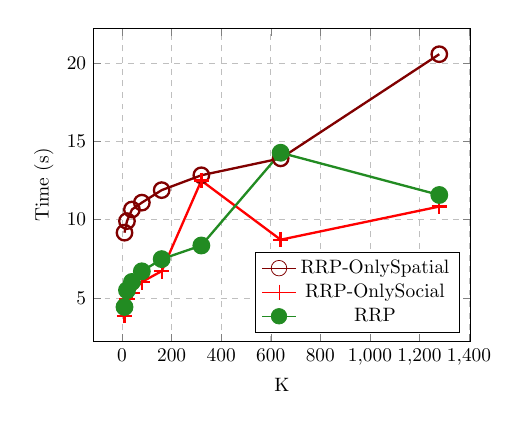
\begin{tikzpicture}[every plot/.append style={very thick}, scale=0.70]
			\begin{axis}[
			    xlabel={K},
			    ylabel={Time (s)},
			    legend pos=south east,
			    xmajorgrids=true,
			    ymajorgrids=true,
			    grid style=dashed,
			    mark size=4pt
			]
			 
			% \addplot[
			%     color=blue,
			%     mark=x,
			%     ]
			%     coordinates {
			%     (10,25.67)(20,29.75)(40,25.14)(80,30.61)(160,24.84)(320,24.94)(640,24.95)(1280,24.94)
			%     };
			\addplot[
			    color=Maroon,
			    mark=o,
			    ]
			    coordinates {
			    (10,9.17)(20,9.91)(40,10.65)(80,11.09)(160,11.89)(320,12.84)(640,13.92)(1280,20.58)
			    };
			\addplot[
			    color=red,
			    mark=+,
			    ]
			    coordinates {
				(10,3.86)(20,4.93)(40,5.33)(80,6.02)(160,6.71)(320,12.5)(640,8.72)(1280,10.84)
			    };
			\addplot[
			    color=ForestGreen,
			    mark=*,
			    ]
			    coordinates {
			    (10,4.42)(20,5.49)(40,6.02)(80,6.7)(160,7.48)(320,8.35)(640,14.28)(1280,11.58)
			    };
			    % \legend{DisjointSearch, RRP-OnlySpatial, RRP-OnlySocial, RRP}
			    \legend{RRP-OnlySpatial, RRP-OnlySocial, RRP}
			 
			\end{axis}
		\end{tikzpicture}
		% \caption{Runtime comparison between DisjointSearch and types of RRP algorithms using VertexReachAlgo Type 1 and RZ = 100}
		\caption{Runtime comparison between the types of RRP algorithms using VertexReachAlgo Type 1 and RZ = 100}
		\label{fig:plot-04}
	\end{subfigure}
	\begin{subfigure}[t]{0.33\textwidth}
		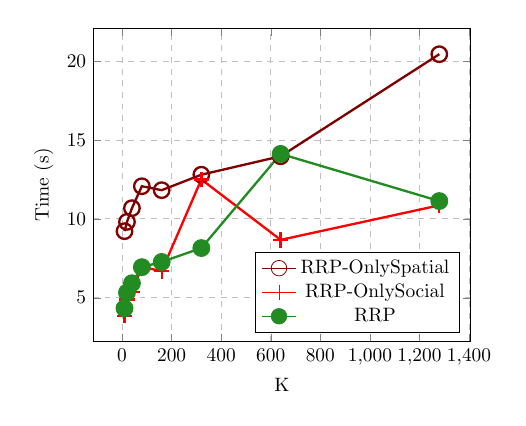
\begin{tikzpicture}[every plot/.append style={very thick}, scale=0.70]
			\begin{axis}[
			    xlabel={K},
			    ylabel={Time (s)},
			    legend pos=south east,
			    xmajorgrids=true,
			    ymajorgrids=true,
			    grid style=dashed,
			    mark size=4pt
			]
			 
			% \addplot[
			%     color=blue,
			%     mark=x,
			%     ]
			%     coordinates {
			%     (10,26.11)(20,30.17)(40,25.41)(80,29.98)(160,25.37)(320,24.77)(640,25.03)(1280,24.82)
			%     };
			\addplot[
			    color=Maroon,
			    mark=o,
			    ]
			    coordinates {
			    (10,9.22)(20,9.81)(40,10.68)(80,12.07)(160,11.82)(320,12.8)(640,13.97)(1280,20.44)
			    };
			\addplot[
			    color=red,
			    mark=+,
			    ]
			    coordinates {
				(10,3.86)(20,4.88)(40,5.36)(80,6.95)(160,6.69)(320,12.5)(640,8.67)(1280,10.86)
			    };
			\addplot[
			    color=ForestGreen,
			    mark=*,
			    ]
			    coordinates {
			    (10,4.33)(20,5.33)(40,5.92)(80,6.94)(160,7.27)(320,8.15)(640,14.12)(1280,11.13)
			    };
			    % \legend{DisjointSearch, RRP-OnlySpatial, RRP-OnlySocial, RRP}
			    \legend{RRP-OnlySpatial, RRP-OnlySocial, RRP}
			 
			\end{axis}
		\end{tikzpicture}
		% \caption{Runtime comparison between DisjointSearch and types of RRP algorithms using VertexReachAlgo Type 2 and RZ = 100}
		\caption{Runtime comparison between the types of RRP algorithms using VertexReachAlgo Type 2 and RZ = 100}
		\label{fig:plot-05}
	\end{subfigure}
	\begin{subfigure}[t]{0.33\textwidth}
		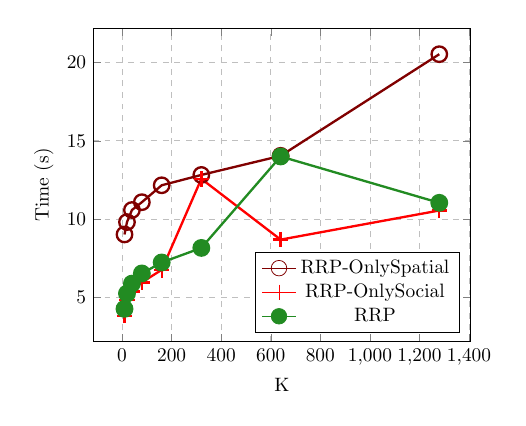
\begin{tikzpicture}[every plot/.append style={very thick}, scale=0.70]
			\begin{axis}[
			    xlabel={K},
			    ylabel={Time (s)},
			    legend pos=south east,
			    xmajorgrids=true,
			    ymajorgrids=true,
			    grid style=dashed,
			    mark size=4pt
			]
			 
			% \addplot[
			%     color=blue,
			%     mark=x,
			%     ]
			%     coordinates {
			%     (10,25.14)(20,29.93)(40,25.51)(80,30.6)(160,24.84)(320,24.97)(640,25)(1280,25.09)
			%     };
			\addplot[
			    color=Maroon,
			    mark=o,
			    ]
			    coordinates {
			    (10,9.02)(20,9.81)(40,10.58)(80,11.08)(160,12.16)(320,12.82)(640,14.04)(1280,20.53)
			    };
			\addplot[
			    color=red,
			    mark=+,
			    ]
			    coordinates {
				(10,3.83)(20,4.85)(40,5.37)(80,5.96)(160,6.76)(320,12.57)(640,8.69)(1280,10.55)
			    };
			\addplot[
			    color=ForestGreen,
			    mark=*,
			    ]
			    coordinates {
			    (10,4.27)(20,5.25)(40,5.88)(80,6.53)(160,7.23)(320,8.16)(640,14)(1280,11.04)
			    };
			    % \legend{DisjointSearch, RRP-OnlySpatial, RRP-OnlySocial, RRP}
			    \legend{RRP-OnlySpatial, RRP-OnlySocial, RRP}
			 
			\end{axis}
		\end{tikzpicture}
		% \caption{Runtime comparison between DisjointSearch and types of RRP algorithms using VertexReachAlgo Type 3 and RZ = 100}
		\caption{Runtime comparison between the types of RRP algorithms using VertexReachAlgo Type 3 and RZ = 100}
		\label{fig:plot-06}
	\end{subfigure}
	\caption{Runtime comparison between the types of RRP algorithms for various VertexReachAlgo Types}
\end{figure*}

Now that we know how each algorithm for LIES\_IN is implemented, we can clearly see that from figures \ref{fig:plot-04}, \ref{fig:plot-05}, \ref{fig:plot-06} that all perform the same way. However, if we mash them together keeping the K constant, we see that Algorithm of Type 3 outperforms in most cases. This confirms the previous doubt that if the resolution is too high like 1,000 by 1,000 the overhead in LIES\_IN function overcomes the advantage gained by graph pruning in a dense graph. Now to figure out the sweet spot for right value of RZ, we perform experiments comparing K VS Resolution VS Time for each variant of RRP. 

\begin{figure*}[t]
	\begin{subfigure}[t]{0.5\textwidth}
		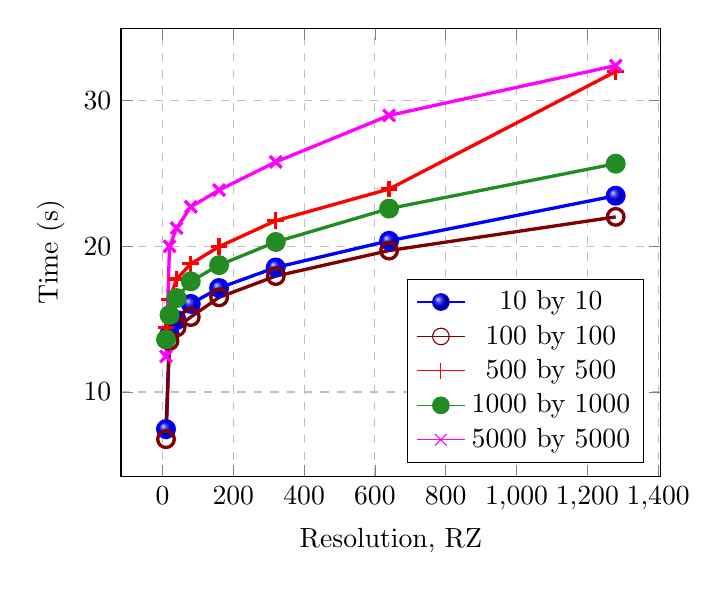
\begin{tikzpicture}[every plot/.append style={very thick}][scale=0.85]
			\begin{axis}[
			    xlabel={Resolution, RZ},
			    ylabel={Time (s)},
			    legend pos=south east,
			    xmajorgrids=true,
			    ymajorgrids=true,
			    grid style=dashed,
			    mark size=3pt
			]
			 
			\addplot[
			    color=blue,
			    mark=ball,
			    ]
			    coordinates {
			    (10.0, 7.45)(20.0, 13.99)(40.0, 14.93)(80.0, 16.04)(160.0, 17.13)(320.0, 18.54)(640.0, 20.37)(1280.0, 23.46)
			    };
			\addplot[
			    color=Maroon,
			    mark=o,
			    ]
			    coordinates {
			    (10.0, 6.76)(20.0, 13.5)(40.0, 14.43)(80.0, 15.14)(160.0, 16.49)(320.0, 17.95)(640.0, 19.7)(1280.0, 22.01)
			    };
			\addplot[
			    color=red,
			    mark=+,
			    ]
			    coordinates {
				(10.0, 14.44)(20.0, 16.36)(40.0, 17.74)(80.0, 18.79)(160.0, 19.97)(320.0, 21.75)(640.0, 23.92)(1280.0, 31.98)
			    };
			\addplot[
			    color=ForestGreen,
			    mark=*,
			    ]
			    coordinates {
			    (10.0, 13.6)(20.0, 15.28)(40.0, 16.44)(80.0, 17.59)(160.0, 18.7)(320.0, 20.29)(640.0, 22.58)(1280.0, 25.66)
			    };
			\addplot[
			    color=Magenta,
			    mark=x,
			    ]
			    coordinates {
			    (10.0, 12.44)(20.0, 19.99)(40.0, 21.24)(80.0, 22.7)(160.0, 23.85)(320.0, 25.78)(640.0, 28.97)(1280.0, 32.39)
			    };
			    \legend{10 by 10,100 by 100,500 by 500,1000 by 1000,5000 by 5000}
			 
			\end{axis}
		\end{tikzpicture}
		\caption{Runtime comparison between Resolution and K using only SpatialIndex of RRP}
		\label{fig:plot-07}
	\end{subfigure}
	\begin{subfigure}[t]{0.5\textwidth}
		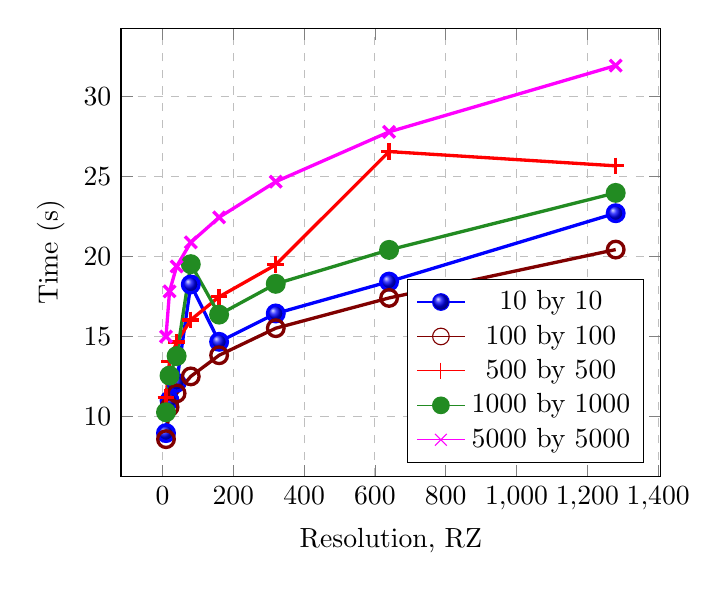
\begin{tikzpicture}[every plot/.append style={very thick}][scale=0.85]
			\begin{axis}[
			    xlabel={Resolution, RZ},
			    ylabel={Time (s)},
			    legend pos=south east,
			    xmajorgrids=true,
			    ymajorgrids=true,
			    grid style=dashed,
			    mark size=3pt
			]
			 
			\addplot[
			    color=blue,
			    mark=ball,
			    ]
			    coordinates {
			    (10.0, 8.98)(20.0, 11.02)(40.0, 12.12)(80.0, 18.26)(160.0, 14.68)(320.0, 16.45)(640.0, 18.44)(1280.0, 22.71)
			    };
			\addplot[
			    color=Maroon,
			    mark=o,
			    ]
			    coordinates {
			    (10.0, 8.6)(20.0, 10.6)(40.0, 11.46)(80.0, 12.52)(160.0, 13.84)(320.0, 15.53)(640.0, 17.42)(1280.0, 20.44)
			    };
			\addplot[
			    color=red,
			    mark=+,
			    ]
			    coordinates {
				(10.0, 11.2)(20.0, 13.47)(40.0, 14.66)(80.0, 16.05)(160.0, 17.49)(320.0, 19.49)(640.0, 26.56)(1280.0, 25.67)
			    };
			\addplot[
			    color=ForestGreen,
			    mark=*,
			    ]
			    coordinates {
			    (10.0, 10.28)(20.0, 12.57)(40.0, 13.79)(80.0, 19.53)(160.0, 16.38)(320.0, 18.3)(640.0, 20.42)(1280.0, 23.98)
			    };
			\addplot[
			    color=Magenta,
			    mark=x,
			    ]
			    coordinates {
			    (10.0, 15.01)(20.0, 17.83)(40.0, 19.39)(80.0, 20.89)(160.0, 22.45)(320.0, 24.68)(640.0, 27.79)(1280.0, 31.93)
			    };
			    \legend{10 by 10,100 by 100,500 by 500,1000 by 1000,5000 by 5000}
			 
			\end{axis}
		\end{tikzpicture}
		\caption{Runtime comparison between Resolution and K using both Social+Spatial indices of RRP}
		\label{fig:plot-08}
	\end{subfigure}
	\caption{Runtime comparison between Resolution and K for different types of RRP algorithms}
\end{figure*}

From Figure \ref{fig:plot-07} we can see that as resolution increases for a fixed K and Spatial Index variant of RRP, performance degrades for very high resolutions due to the overhead by LIES\_IN function. For very low resolutions, as each block is almost the size of Texas, even if a user checks-in at one restaurant there, he/she is considered reachable to that block. So it turns many vertices can reach majority of the blocks making it less useful to use a spatial index. The sweet spot so is in between the both extremes, which is 100 in this case. Similar conclusions can be made in next case \ref {fig:plot-08} where both indices are used. The humps are due to the inefficiency of the landmark and nothing to do with Spatial Index.

So after these experiments, we find that when the graph is really dense using the social index with a high quality landmark is sufficient. Now let us see how things change when the quality of landmark(s) is not as good. For the next query, the region is even more densely connected and the source vertex is the same, however we fed a moderate quality landmark. This region has 21,239 spatial nodes which is almost 10 times the count of the previous one.

Figure \ref{fig:plot-09} proves why just having a social index wont help like before. For this region, we purposefully chose a moderate landmark. In such cases spatial index prunes majority of the graph as we have a decent resolution of 100 by 100. Though social index outperformed social+spatial index, it lost soon as the landmark wasn't good enough. The correctness is never compromised, it is only that RRP tends to Dijkstra's search if landmark quality is not good. Now that we are convinced when to use each type of index, let us see how each of our algorithms perform with change in region size.

\begin{figure*}[t]
\begin{subfigure}[t]{0.5\textwidth}
	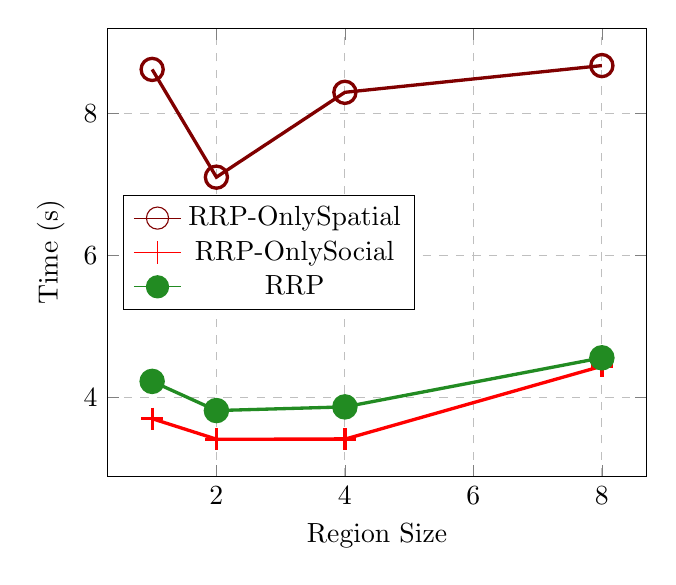
\begin{tikzpicture}[every plot/.append style={very thick}][scale=0.85]
		\begin{axis}[
		    xlabel={Region Size},
		    ylabel={Time (s)},
		    % legend pos=south west,
		    legend style={at={(0.03,0.5)},anchor=west},
		    % legend style={at={(0,-0.1)},anchor=north},
		    xmajorgrids=true,
		    ymajorgrids=true,
		    grid style=dashed,
		    mark size=4pt
		]
		 
		% \addplot[
		%     color=blue,
		%     mark=x,
		%     ]
		%     coordinates {
		%     (1, 25.81058407)(2, 30.50130916)(4, 31.07799816)(8, 32.95914412)
		%     };
		\addplot[
		    color=Maroon,
		    mark=o,
		    ]
		    coordinates {
		    (1, 8.615309954)(2, 7.099899054)(4, 8.293120861)(8, 8.6691780567)
		    };
		\addplot[
		    color=red,
		    mark=+,
		    ]
		    coordinates {
		    (1, 3.703080177)(2, 3.414629221)(4, 3.415085077)(8, 4.441617966)
		    };
		\addplot[
		    color=ForestGreen,
		    mark=*,
		    ]
		    coordinates {
		    (1, 4.227499962)(2, 3.817003012)(4, 3.868695974)(8, 4.559159994)
		    };
		    % \legend{DisjointSearch, RRP-OnlySpatial, RRP-OnlySocial, RRP}
		    \legend{RRP-OnlySpatial, RRP-OnlySocial, RRP}
		 
		\end{axis}
	\end{tikzpicture}
	% \caption{Runtime comparison between DisjointSearch and types of RRP algorithms for changes in region size for a source vertex S1}
	\caption{Runtime comparison between types of RRP algorithms for changes in region size for a source vertex S1}
	\label{fig:plot-10}
\end{subfigure}
\begin{subfigure}[t]{0.5\textwidth}
	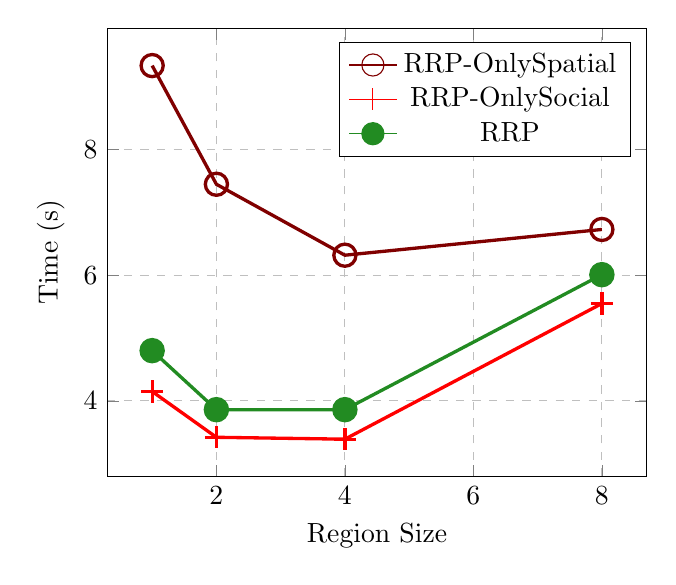
\begin{tikzpicture}[every plot/.append style={very thick}][scale=0.85]
		\begin{axis}[
		    xlabel={Region Size},
		    ylabel={Time (s)},
		    legend pos=north east,
		    xmajorgrids=true,
		    ymajorgrids=true,
		    grid style=dashed,
		    mark size=4pt
		]
		 
		% \addplot[
		%     color=blue,
		%     mark=x,
		%     ]
		%     coordinates {
		%     (1, 26.25)(2, 30.53)(4, 30.52)(8, 32.17)
		%     };
		\addplot[
		    color=Maroon,
		    mark=o,
		    ]
		    coordinates {
		    (1, 9.34)(2, 7.45)(4, 6.32)(8, 6.73)
		    };
		\addplot[
		    color=red,
		    mark=+,
		    ]
		    coordinates {
		    (1, 4.15)(2, 3.42)(4, 3.39)(8, 5.55)
		    };
		\addplot[
		    color=ForestGreen,
		    mark=*,
		    ]
		    coordinates {
		    (1, 4.8)(2, 3.86)(4, 3.86)(8, 6.01)
		    };
		    % \legend{DisjointSearch, RRP-OnlySpatial, RRP-OnlySocial, RRP}
		    \legend{RRP-OnlySpatial, RRP-OnlySocial, RRP}
		 
		\end{axis}
	\end{tikzpicture}
	% \caption{Runtime comparison between DisjointSearch and types of RRP algorithms for changes in region size for a source vertex S2}
	\caption{Runtime comparison between the types of RRP algorithms for changes in region size for a source vertex S2}
	\label{fig:plot-11}
\end{subfigure}
\caption{Runtime comparison between the types of RRP algorithms for changes in region size for different source verteices}
\end{figure*}

In Figure \ref{fig:plot-10} we can see how every algorithm linearly increase the time taken w.r.t. the size of the region. Here the source vertex has many check-ins in each region and so the spatial index performs worse initially due to its overhead but gradually performs better than social and social+spatial indices as the size of the region increases. This is even more evident when we choose a user who doesn't have many check-ins the query regions and has to traverse the social graph to find paths as shown in Figure \ref{fig:plot-11}.
